\section{Operating Charts}
Operating charts describe the modes of operation and the flow of the system without much detail. Figure~\ref{fig:systemFlowchart} shows the system's main flowchart, which depicts how the device goes in and out of each of its operating modes.  A general but brief overview of the different modes of operation follows.

When the system is powered up it will perform an initialization sequence, which includes initializing all GPIO ports and memory variables. It will also enable global interrupts and the RF wakeup receiver interrupt while keeping all other interrupts disabled. It will also power down all other modules while keeping the RF wakeup receiver on.
When the initialization sequence is finished, it will enter a very low power mode. This mode will be called shutdown mode. The system can be woken up by the RF wakeup receiver which will be listening for a specific signal from the user. When the system is interrupted from sleep by the RF wakeup receiver it will power on the XBee module, establish a Zigbee connection, and enable the Xbee interrupt. Also, the system will power off the RF wakeup receiver and disable its corresponding interrupt.
Afterwards, the system will enter in another low power mode which will be referred to as standby mode. In this mode, the system will maintain an active Zigbee connection via the Xbee module. The Xbee module will be listening for specific signal from the base station. When it receives a signal, it will interrupt the MCU and set a flag corresponding to the signal that was received. The signal could be to enter either diagnostic, retrieval, sampling, status, or shutdown mode, or to exit diagnostic mode. The interrupt routine will then take the CPU to active mode, and the system will proceed to execute the service corresponding to the signal that was sent to the XBee module via the base station. After the service has finished executing, the system will return to standby mode where it will listen for more incoming commands.

The following sections contain a more thorough explanation of each of the operating modes mentioned, along with a flowchart of its own to help explain what can be done in each mode.
\begin{figure}[H]
	\centering
	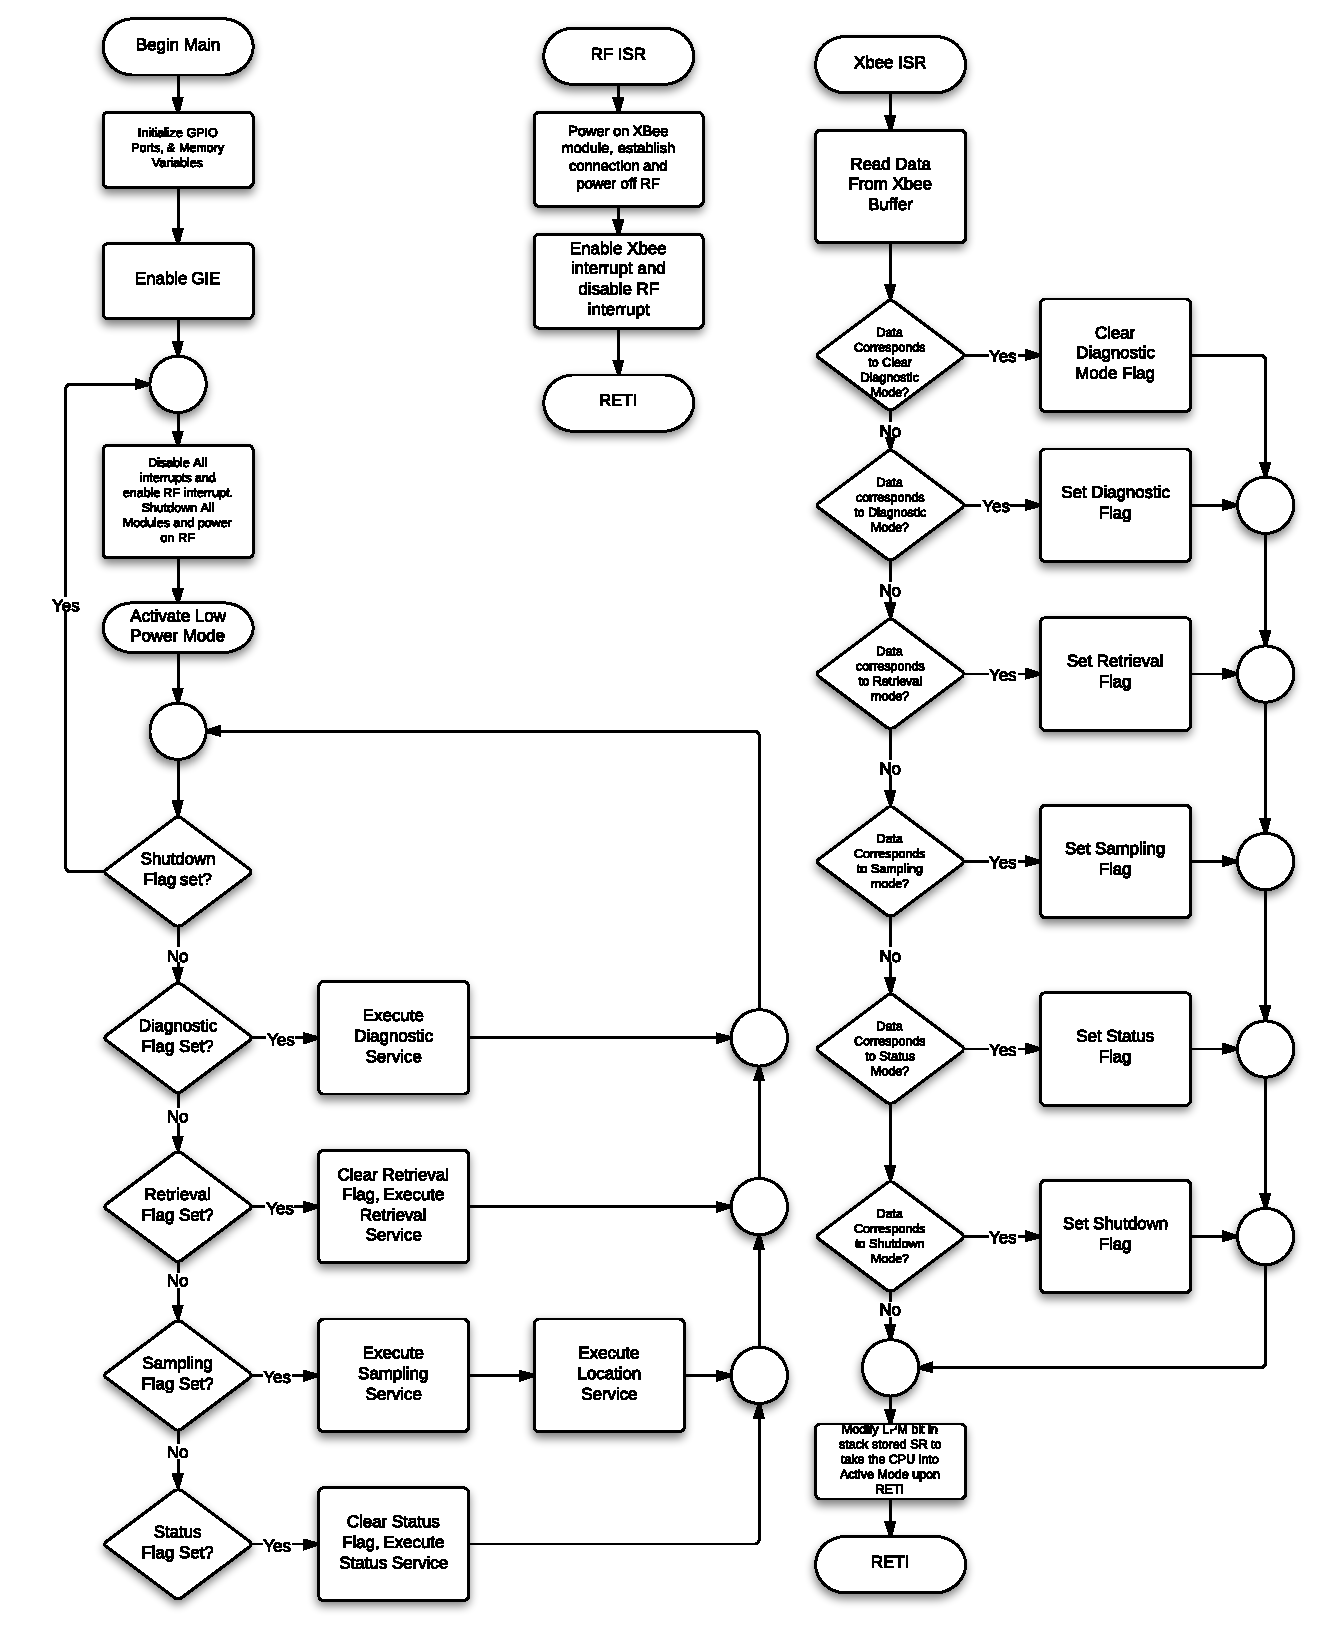
\includegraphics[scale=0.8]{img/SystemFlowchart}
	\caption{System Operating Chart \label{fig:systemFlowchart}}
\end{figure}

\subsection{Diagnostic Event Service}
In this service, which will be called Diagnostic Mode, the device maintains communication to the base station and sends real-time measurement information of the different components to the base station. The user can then observe and verify that all components are taking accurate measurements and that data can be retrieved through the XBee module. If the user decides to exit Diagnostic mode, he will do so by choosing the option at the base station, which will send the corresponding signal to the Xbee module and interrupt the MCU. The Diagnostic flag will be cleared by the interrupt routine, and will cause the return of the Diagnostic Event Service, shown below.
\begin{figure}[H]
	\centering
	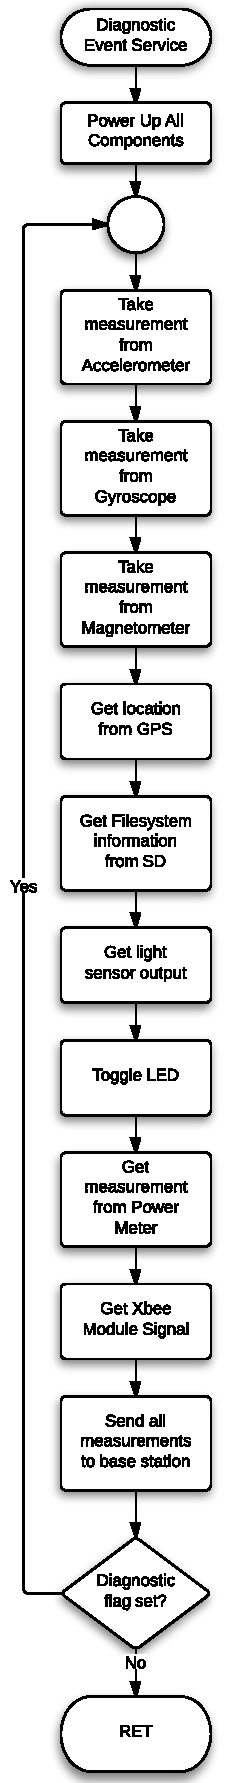
\includegraphics[scale=0.7]{img/DiagnosticEventService}
	\caption{Flowchart for Diagnostic Event Service \label{fig:diagnosticMode}}
\end{figure}

\subsection{Retrieval Event Service}
Retrieval Mode is the operation mode of the device in which the system transfers the data collected while in Sampling Mode. This data from the SD Card to the base station. Data is transferred trough the established ZigBee connection and once all data has been transferred it is erased from the SD card.
\begin{figure}[H]
	\centering
	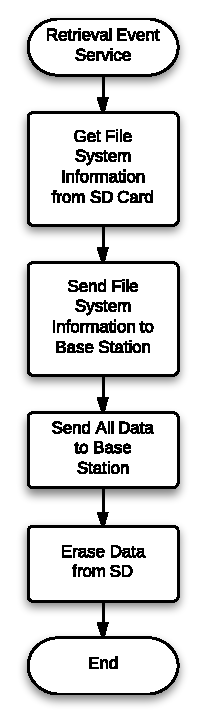
\includegraphics[scale=1.0]{img/RetrievalEventService}
	\caption{Flowchart for Retrieval Event Service \label{fig:retrivalMode}}
\end{figure}


\subsection{Sampling Event Service}
While in Sampling Mode the device captures data from the accelerometer, gyroscope and magnetometer. Data is captured for 30 seconds and data points are saved in the SD card, each with a time stamp from the time which they were captured. The data will be sampled at 256Hz. This frequency will be fulfilled by using a timer with a crystal oscillator.
\begin{figure}[H]
	\centering
	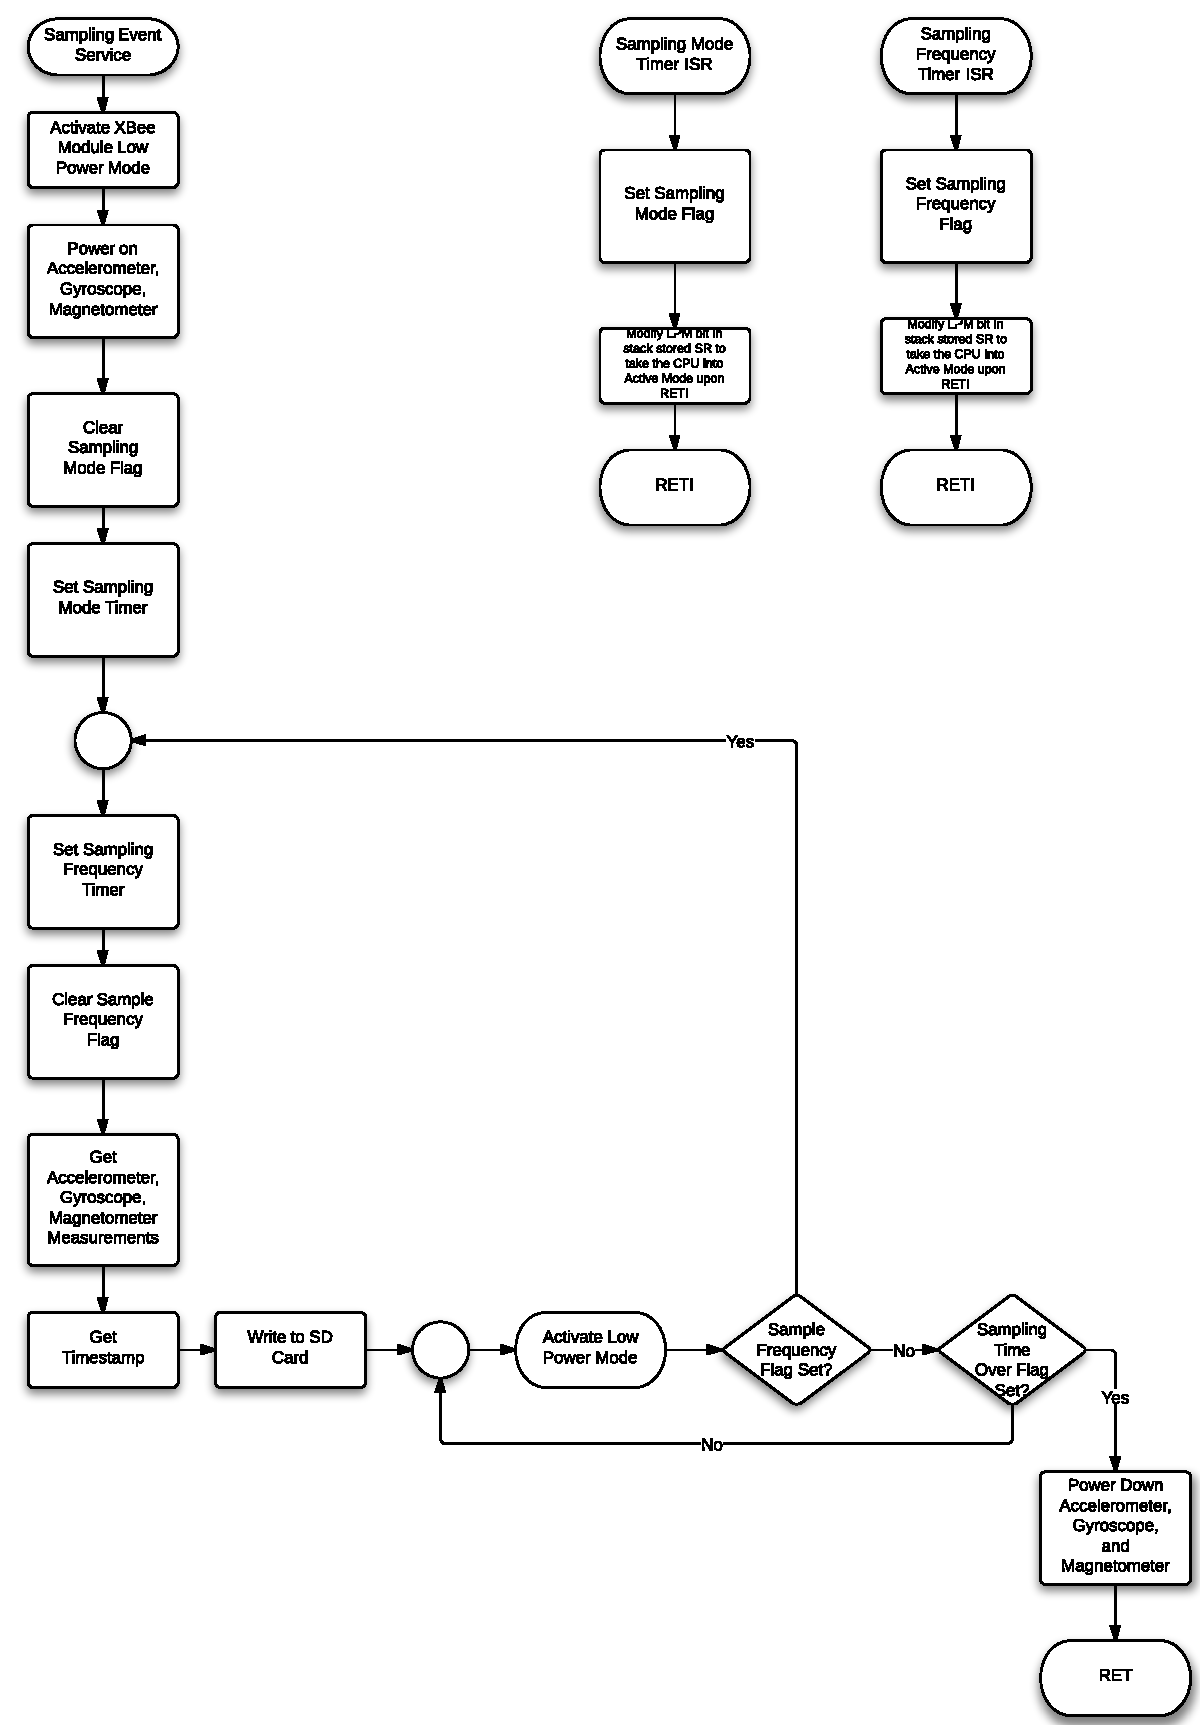
\includegraphics[scale=0.7]{img/SamplingEventService}
	\caption{Flowchart for Sampling Event Service \label{fig:samplingMode}}
\end{figure}

\subsection{Location Event Service}
On Locate Mode the user is trying find and retrieve the device. The system turns on the XBee Module and the GPS. The system then proceeds to establishing a ZigBee connection to the base station and get a GPS lock. Once the device gets its location using the GPS Module it will then broadcast the location to the base station through the ZigBee connection.
\begin{figure}[H]
	\centering
	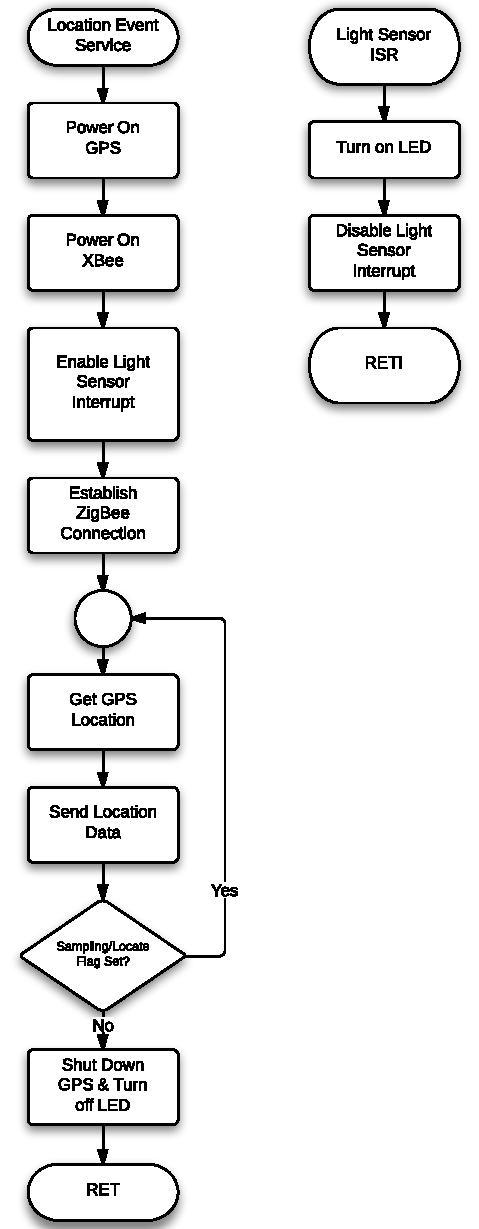
\includegraphics[scale=1.0]{img/LocationEventService}
	\caption{Flowchart for Location Event Service \label{fig:locateMode}}
\end{figure}

\subsection{Status Event Service}
The status event service will send battery charge status and SD card information to the base station. The SD card information includes free space and file system information.
\begin{figure}[H]
	\centering
	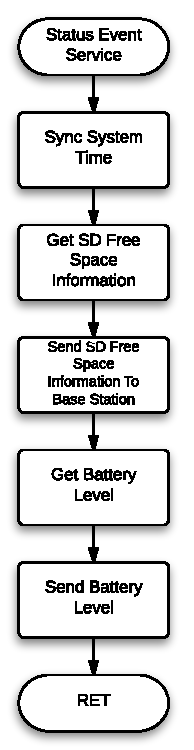
\includegraphics[scale=1.0]{img/StatusEventService}
	\caption{Flowchart for Status Event Service \label{fig:statusMode}}
\end{figure}